\documentclass[../main.tex]{subfiles}

\begin{document}
    \subsection{Grafiken zu Lab 2}
    Während dem Durchlauf des Experimentes des Lab 2, werden diverse Daten physikalische Vorgängen
    gesammelt. Diese Daten umfassen Ort und Geschwindigkeit, sowie kinetische und potentielle Energie.
    Dabei wird zwischen dem elastischen sowie inelastischen Zusammenstoss unterschieden.
    \subsubsection{Elastisch}
    Nachfolgend werden alle Daten als Funktion der Zeit zu dem elastischen Zusammenstoss in der
    Abbildung~\ref{fig:GeschwindigkeitAlsFunktionDerZeit} bis Abbildung~\ref{fig:OrtAlsFunktionDerZeit}
    aufgegliedert.

    \begin{figure}[H]
        \begin{center}
            \centerline{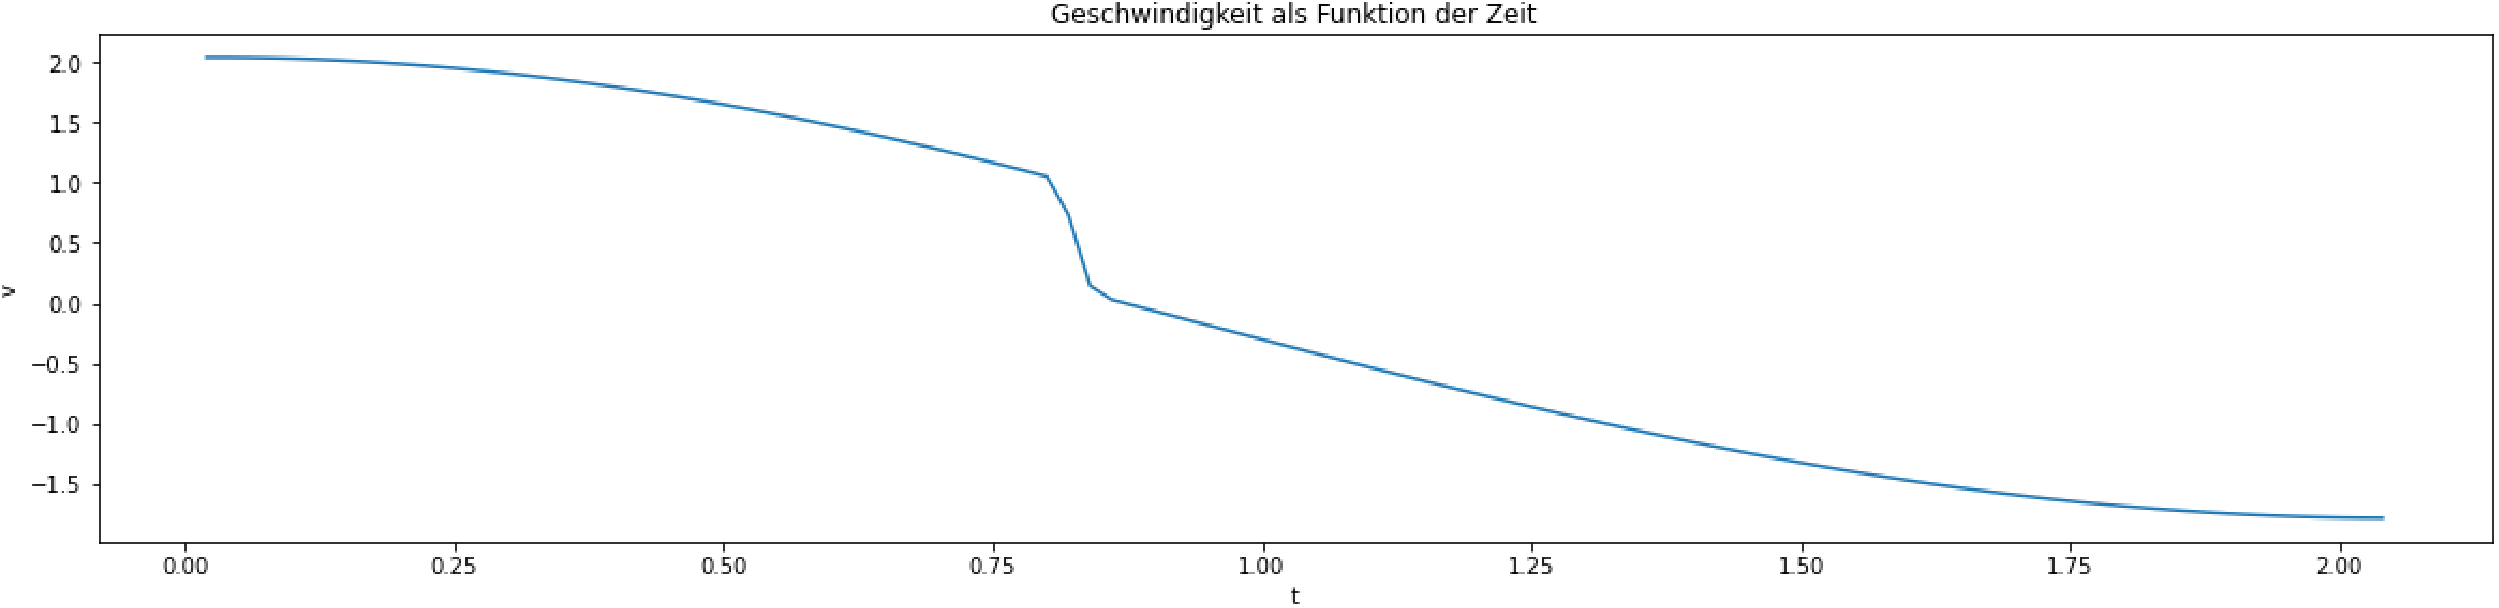
\includegraphics[width=105mm]{./images/Elastisch/GeschwindigkeitAlsFunktionDerZeit}}
            \caption{Geschwindigkeit als Funktion der Zeit}
            \label{fig:GeschwindigkeitAlsFunktionDerZeit}
        \end{center}
    \end{figure}

    \begin{figure}[H]
        \begin{center}
            \centerline{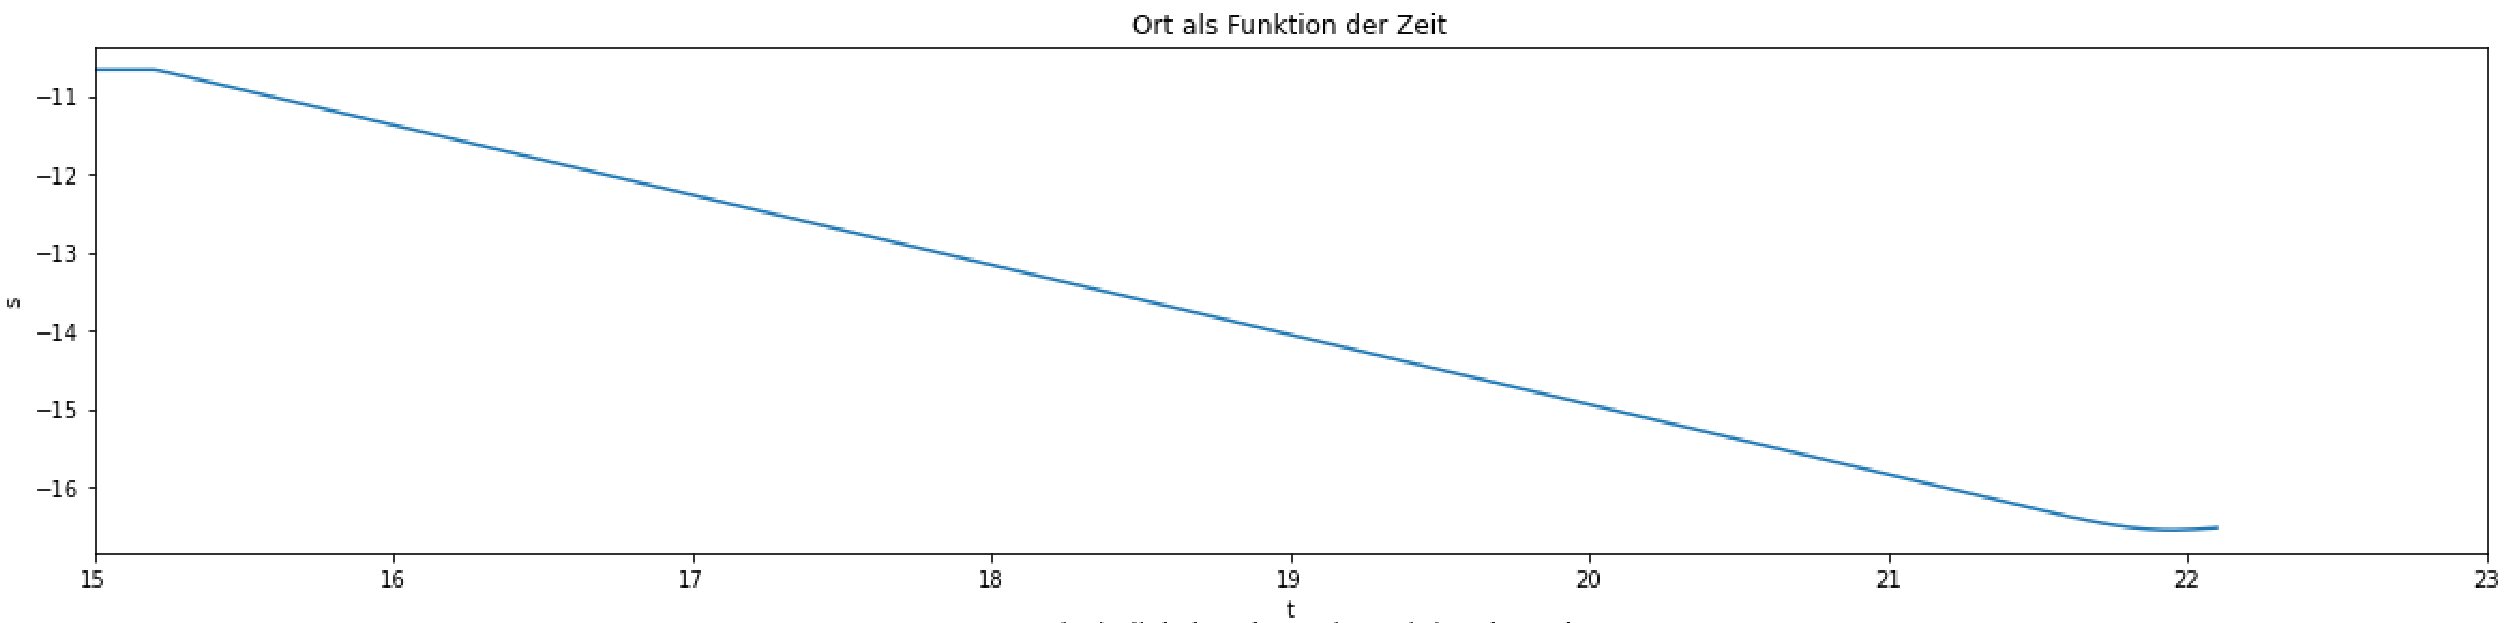
\includegraphics[width=105mm]{./images/Elastisch/OrtAlsFunktionDerZeit}}
            \caption{Ort als Funktion der Zeit}
            \label{fig:OrtAlsFunktionDerZeit}
        \end{center}
    \end{figure}

    \newpage
    \subsubsection{Inelastisch}
    Nachfolgend werden alle Daten als Funktion der Zeit zu dem inelastischen Zusammenstoss in der
    Abbildung~\ref{fig:gesamtImpluls} bis Abbildung~\ref{fig:Endgeschwindigkeit}
    aufgegliedert.

    \begin{figure}[H]
        \begin{center}
            \centerline{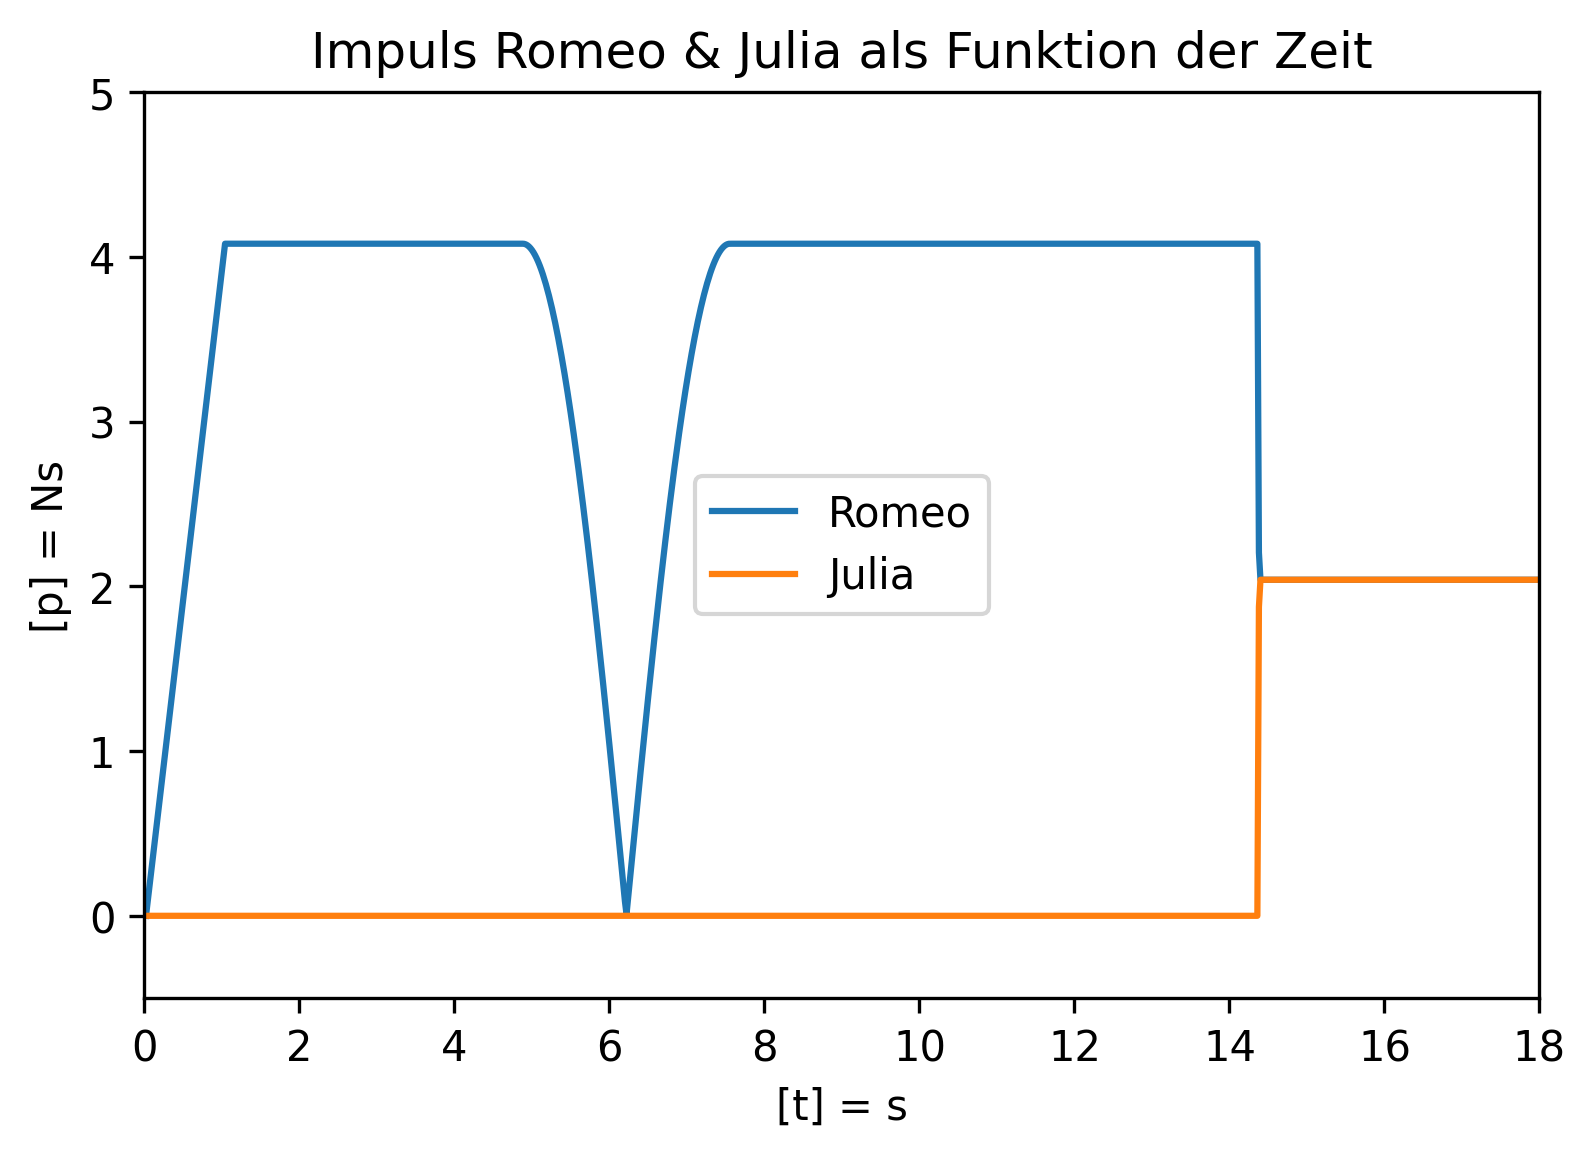
\includegraphics[width=105mm]{./images/Inelastisch/ImpulsRomeoJulia}}
            \caption{Impuls Romeo \& Julia als Funktion der Zeit}
            \label{fig:ImpulsRomeoJulia}
        \end{center}
    \end{figure}

    \begin{figure}[H]
        \begin{center}
            \centerline{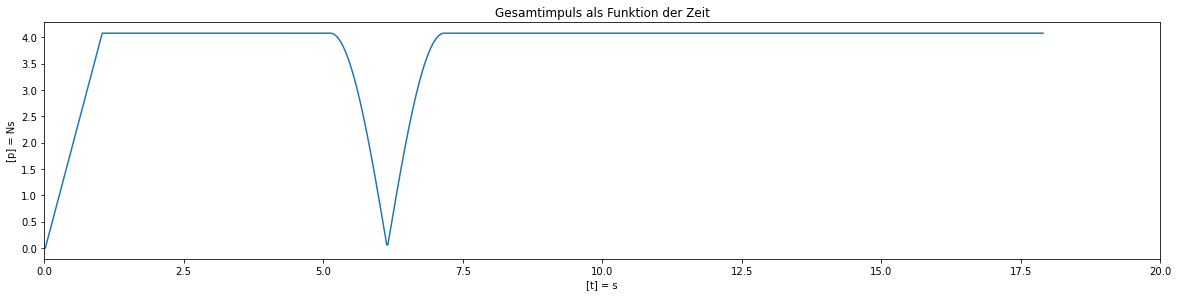
\includegraphics[width=105mm]{./images/Inelastisch/GesamtImpluls}}
            \caption{GesamtImpluls als Funktion der Zeit}
            \label{fig:gesamtImpluls}
        \end{center}
    \end{figure}

    \begin{figure}[H]
        \begin{center}
            \centerline{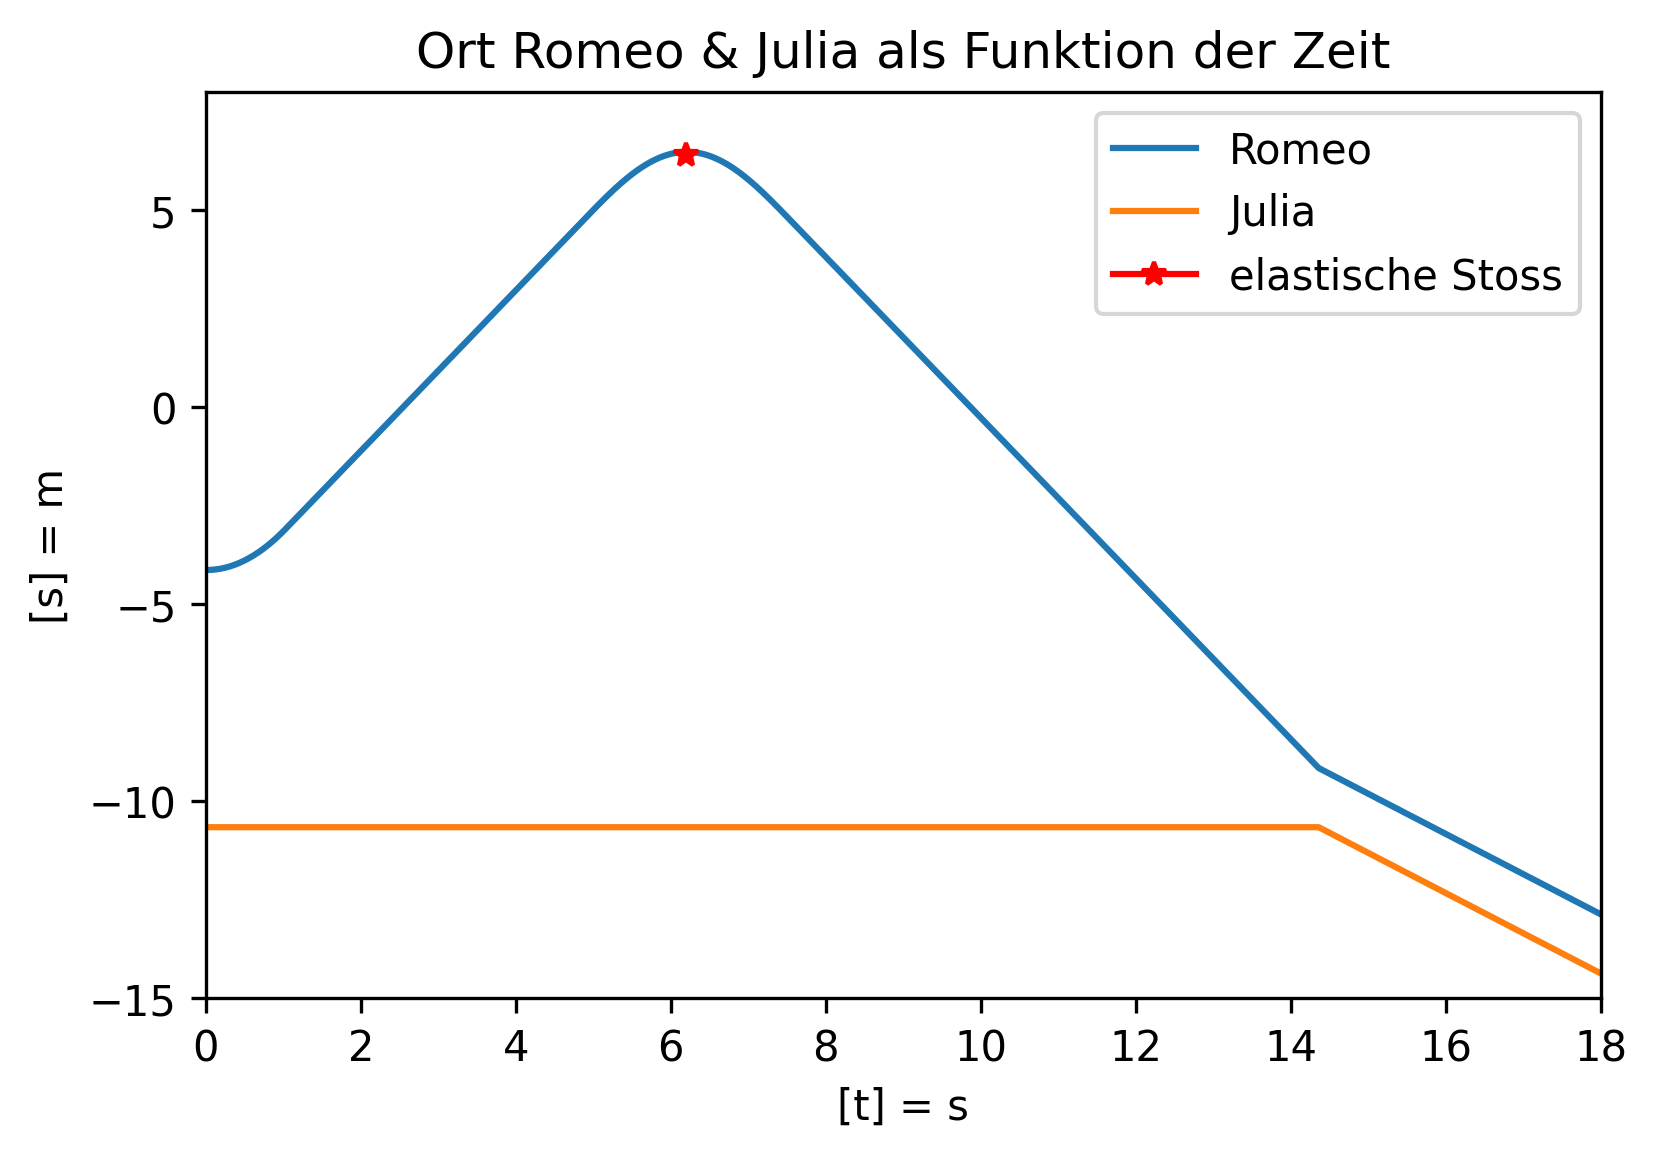
\includegraphics[width=105mm]{./images/Inelastisch/OrtRomeoJuliaAlsFunktionDerZeit}}
            \caption{Ort Romeo \& Julia als Funktion der Zeit}
            \label{fig:OrtRomeoJuliaAlsFunktionDerZeit}
        \end{center}
    \end{figure}

    \begin{figure}[H]
        \begin{center}
            \centerline{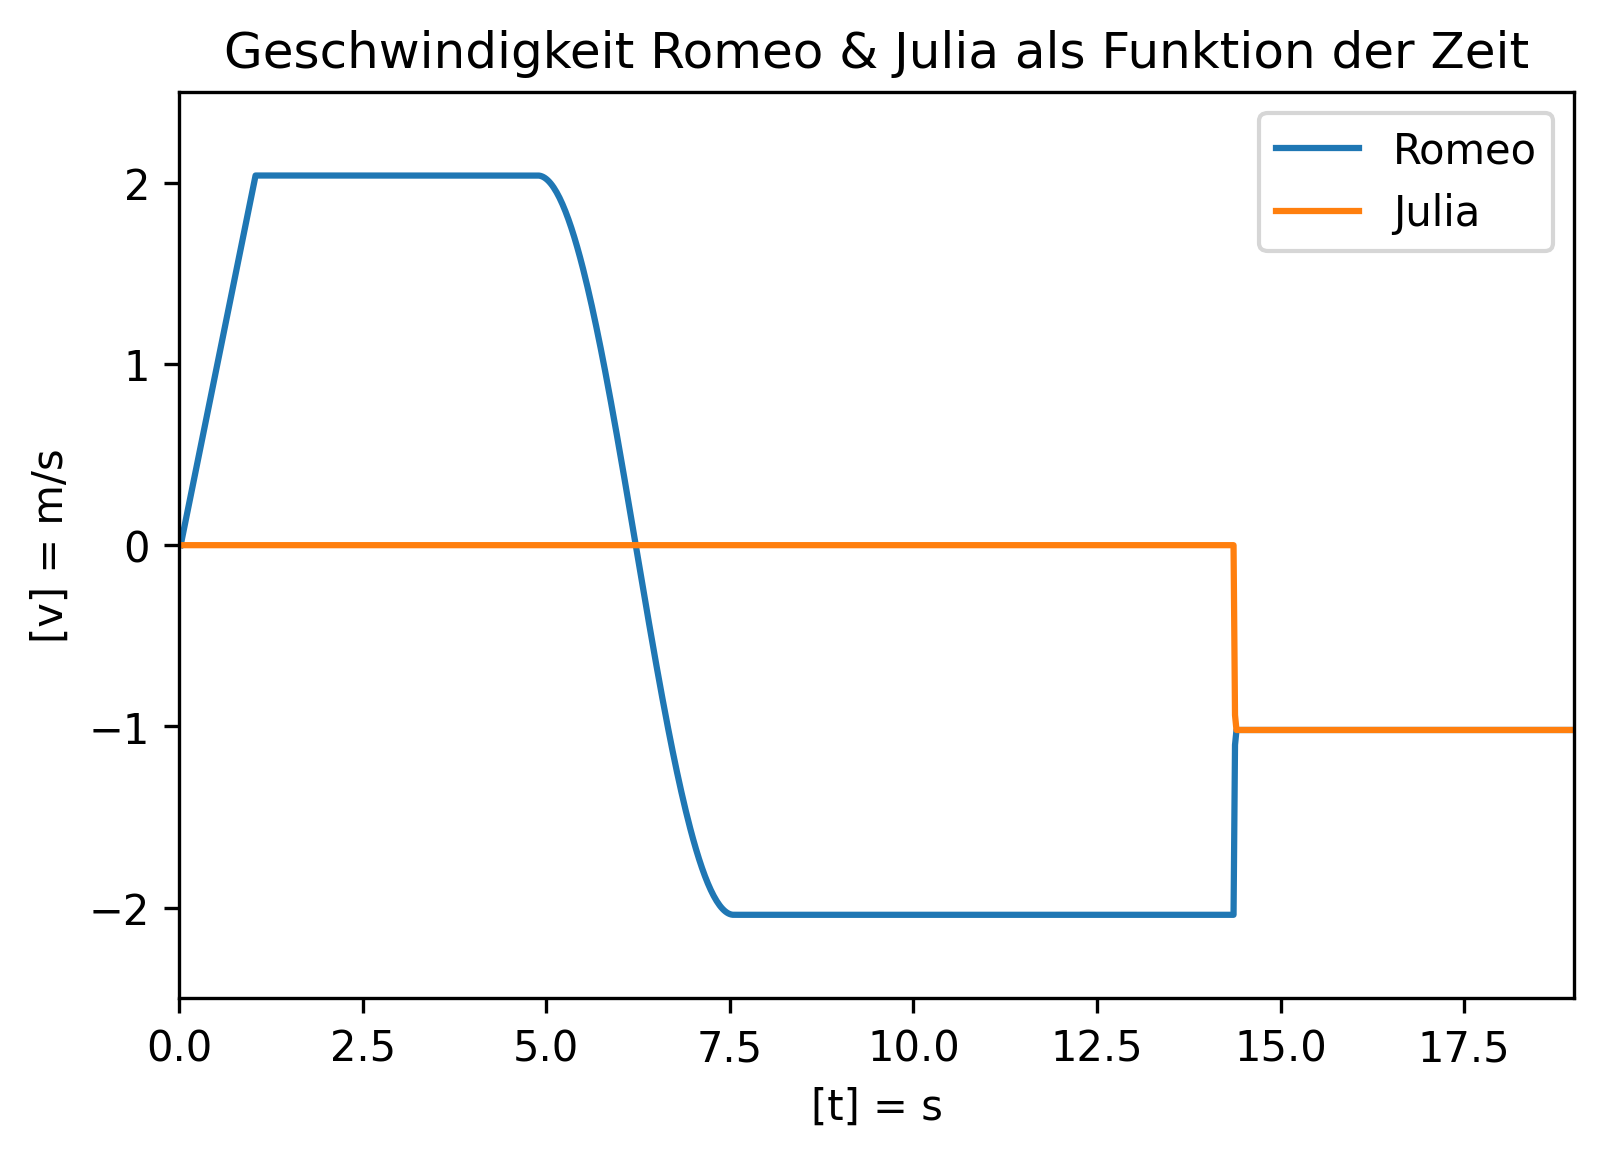
\includegraphics[width=105mm]{./images/Inelastisch/GeschwindigkeitRomeoJulia}}
            \caption{Geschwindigkeit Romeo \& Julia als Funktion der Zeit}
            \label{fig:GeschwindigkeitRomeoJulia}
        \end{center}
    \end{figure}

    \begin{figure}[H]
        \begin{center}
            \centerline{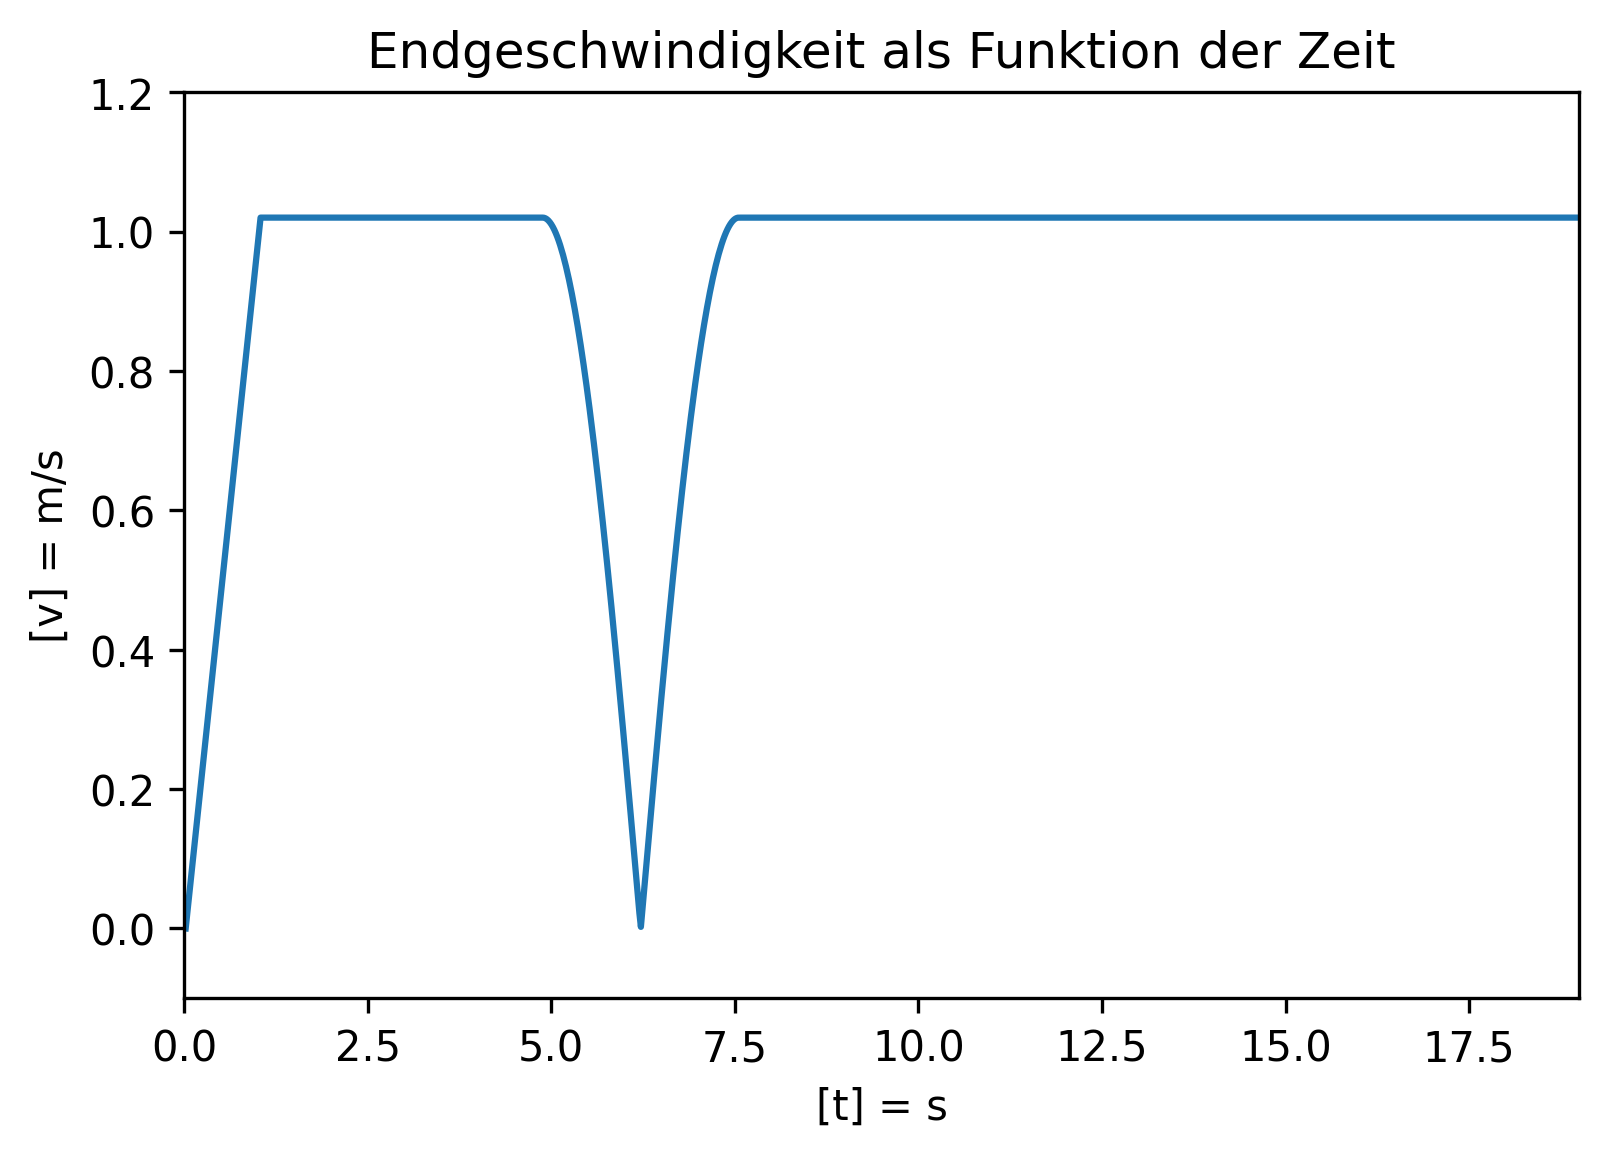
\includegraphics[width=105mm]{./images/Inelastisch/Endgeschwindigkeit}}
            \caption{Endgeschwindigkeit als Funktion der Zeit}
            \label{fig:Endgeschwindigkeit}
        \end{center}
    \end{figure}



\end{document}